%FIX jan 9th, references in this chapter
\section{Quarks, Leptons and Gauge Bosons}%Z radiates a higgs, gluon fushion is dominent production mechanism
%gluons from the colliding beam couple to a heavy quark loop from which the higgs boson is emitted
Following the advances of the 20th century it has been experimentally 
determined that the fundamental
particles in the SM consists of 3 generations of quarks and leptons
where each generation has two particles. 
\begin{figure}[hb]
  \centering
	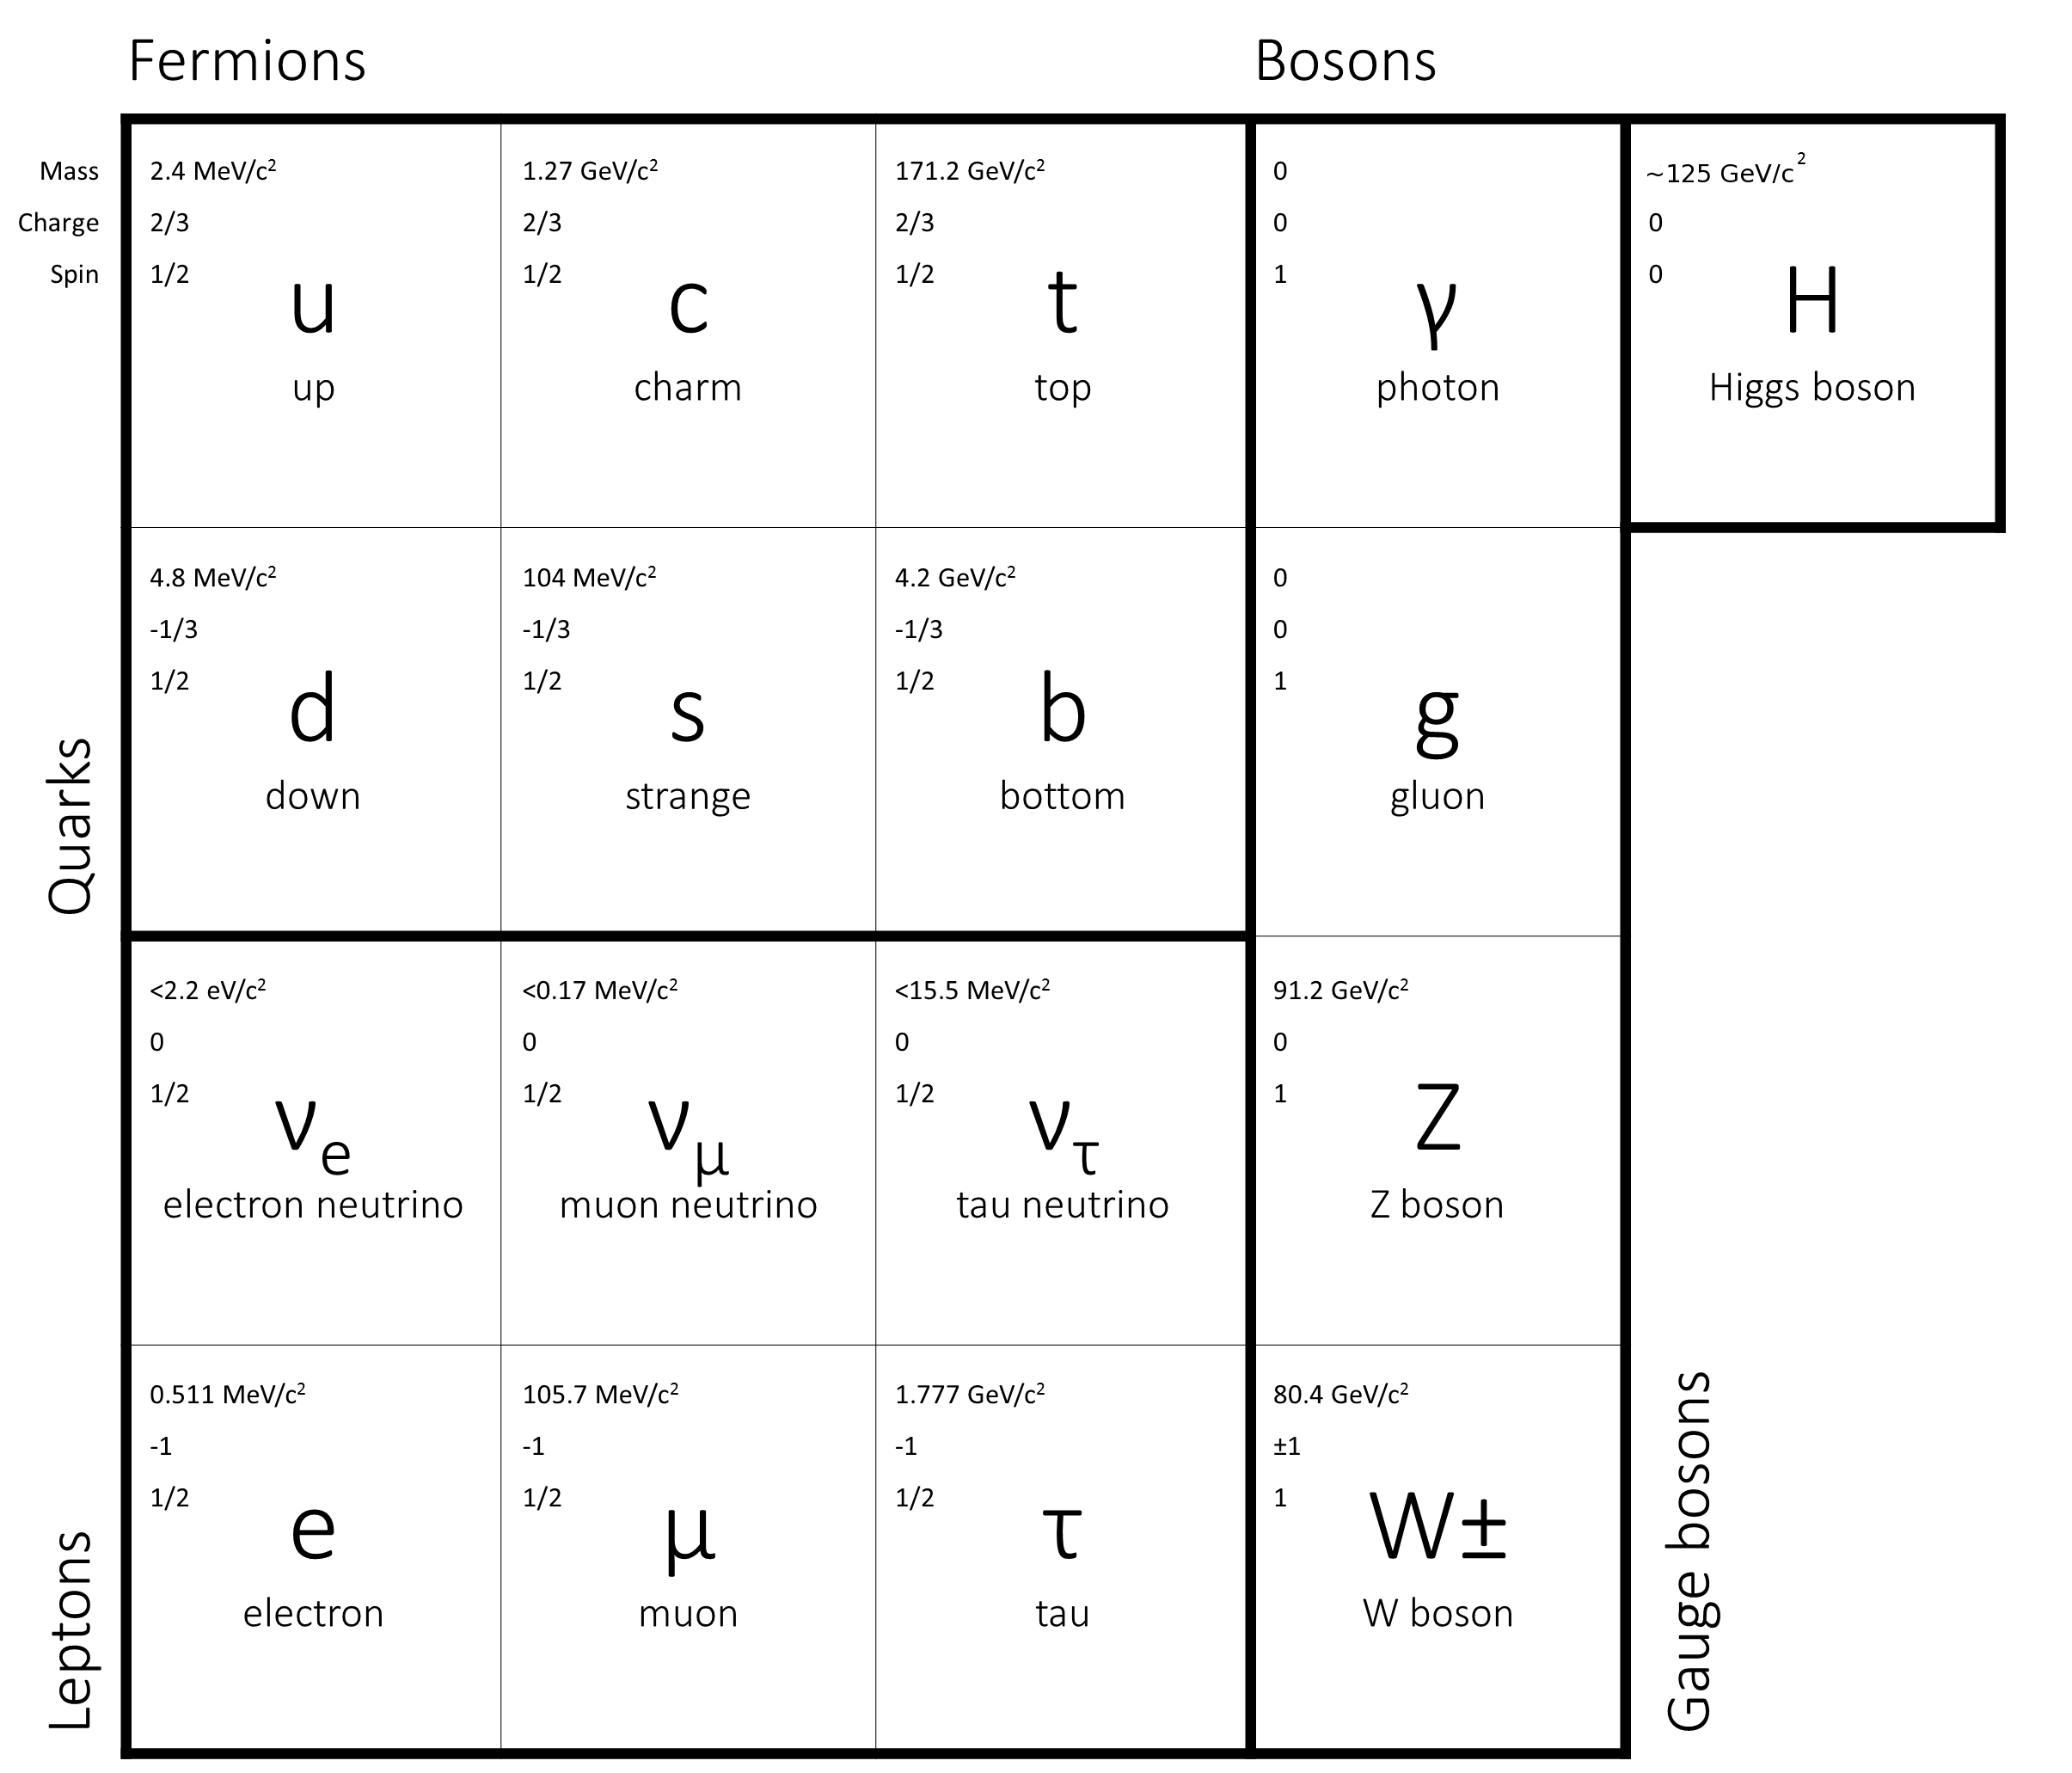
\includegraphics[width=0.6\textwidth]{images/SMParticles2.png}
  	\caption[SM Particles]
   	{Standard Model Particles}
	\label{fig:SMParticles}
\end{figure}
Quarks are spin one-half particles that are triplets of the color group. 
There are 6 flavors of quarks, these are grouped into three generations:
t (top) and b (bottom), c (charm) and s (strange), u (up) and d (down). 
The (u,c,t) quarks have a charge of $\frac{2}{3}$ while the (d,s,b) have 
a charge of $-\frac{1}{3}$.
The fermions (e,$\mu$,$\tau$) all have a charge of -1 while their neutrino 
partners are neutral. Recent experiments in neutrino oscillation have hinted
that neutrinos have a very small mass.
Each fermion has an anti-particle partner with the same mass but opposite charge.
%Starting with the third 
%generation which consists of the heaviest quarks, the top (t) and bottom (b),
%and the $\tau$ lepton and $\tau$ neutrino ($\nu_{\tau}$).
%The second generation consists of the charm (c) and strange (s) quarks,
%the charged muon ($\mu$) and neutral muon neutrino ($\nu_{\mu}$).
%Finally, the first generation which is composed of the lightest 
%quarks, the up (u) and down (d) quarks,
%and the lightest charged lepton with the longest lifetime, the electron (e), and its neutral 
%neutrino partner, the electron neutrino ($\nu_{e}$). 
%The mass, charge and spin can be seen in figure \ref{fig:SMParticles}.
%%%properties, mass, spin, charge, 

Each fundamental force is associated with spin 1 mediator particles.
The weak interactions are mediated by the $W^{\pm}$ and $Z$;
electromagnetic interactions are mediated by the photon and the strong interactions
are mediated by the 8 colored gluons. The Higgs Mechanism (described in the next section) 
is responsible for giving mass to the $W^{\pm}$, $Z$ and the fermions. 
The SM of particle physics describes very successfully the electroweak and strong
interaction of elementary particles over a wide range of energies.

The discovery of a Standard Model Higgs-like boson was announced jointly 
by the CMS and ATLAS collaborations in July of 2012. %%%Cite
As of the writing of this thesis the Higgs Boson has been observed at CMS via
its decay to $ZZ^{*}$, $\gamma\gamma$ and $\tau\tau$. The mass of this
Higgs Boson, as measured by CMS, is 125.6 $\pm$ 0.4(stat.) $\pm$ 0.2(syst.).

The Standard Model of particle physics (SM) follows a $SU(3)\times SU(2)_{L}\times U(1)$ %under field theory??
symmetry. The $SU(2)_{L}\times U(1)$ describes electroweak interactions.
The $SU(3)$ group describes color and the interactions
between gluons and quarks. In the unbroken $SU(2)_{L}\times U(1)$ symmetry
gauge bosons and fermions are massless. However, the recent
discovery of particle that closely resembles the Standard Model Higgs
Boson provides a Mechanism by which the symmetry is broken
and the $W^{\pm}$ and Z bosons, the quarks and leptons acquire mass. 
In the following sections the Higgs Mechanism is described in greater detail.
The extension of the Higgs to the Minimally Supersymmetric Standard Model
is described in the following chapter and the search for it along with
a measurement of the $\Wbb$ cross-section is the main purpose of this
thesis.
\subsection{Background to Lagrangian Construction}%%%Change name?
The idea that interactions are dictated by symmetry is of central
importance to the formulation of theoretical particle physics. 
Currently, it is the general belief that all particle interactions are
described by local gauge theories and that 
physical quantities (charge, color, weakspin, hyper charge) are 
always conserved.
To start the description of SM theory we remember that in classical 
mechanics Lagrange's equations of motion are used to
describe the motion of a particle or system of particles. %%ref goldstein
If we consider the generalized coordinates of a system, $q_{i}$,
and it's derivative as a function of time, $\dot{q_{i}}$, the equation
of motion can be written as,
\begin{equation}
0=\frac{d}{dt}\left(\frac{\partial L}{\partial\dot{q_{i}}}\right) - \frac{\partial L}{\partial q_{i}}
\end{equation}
where $L$ is defined as the difference of the kinetic and the potential energy, $L\equiv T-V$.
This equation can be formally extended to act on a wave function with %%I don't like "act on"
continuously varying coordinates $\phi({\bf x},t)$
where {\bf x} is the spatial coordinates and t is time.
In this regime, the Lagrangian equation of motion becomes
\begin{equation}
0=\frac{\partial}{\partial x_{\mu}}\left( \frac{\La}{\partial\left(\partial\phi/\partial x_{\mu}\right)}\right)-\frac{\partial\La}{\partial\phi}
\end{equation}
In the subsequent sections, following the standard methodology, $\La$ is referred to as the Lagrangian
despite it actually being the Lagrangian density,
\begin{equation}
L=\int{\La d^{3}x}
\end{equation}
To derive the Lagrangian equation of motion for a given interaction
one can easily start from the Feynman Rules.
However, in the following section we take a more formal approach.

\subsection{The Higgs Mechanism and Electroweak Symmetry Breaking}
In this section we illustrate the Higgs Mechanism and partially derive the
Standard Model Lagrangian. 
First we consider the Higgs Mechanism of a global gauge symmetry, 
which the mechanism that generates mass for the gauge bosons. 
We start by writing the Lagrangian, 
\begin{equation}
\La=(\partial_{\mu}\phi)*(\partial^{\mu}\phi) - \mu^{2}\phi*\phi - \lambda (\phi*\phi)^{2}
\label{eq:LU1}
\end{equation}
which describes the complex scalar field, $\phi=(\phi_{1}+i\phi_{2})/\sqrt{2}$.
This Lagrangian is invariant under the phase transformation $\phi\rightarrow e^{i\alpha}\phi$
(which is equivalent to stating that (\ref{eq:LU1}) possesses a $U(1)$ global gauge symmetry).
Here, we consider the case where $\lambda>0$ and $\mu^{2}<0$. To illustrate the importance of (\ref{eq:LU1})
this Lagrangian is rewritten in the form
\begin{equation}
\La \equiv T-V = \frac{1}{2}(\partial_{\mu}\phi_{1})^{2}+\frac{1}{2}(\partial_{\mu}\phi_{2})^{2}-\frac{1}{2}\mu^{2}(\phi_{1}^{2}+\phi_{2}^{2})-\frac{1}{4}\lambda(\phi_{1}^{2}+\phi_{2}^{2})^{2}.
\label{eq:LU2}
\end{equation}
In (\ref{eq:LU2}) the potential term is
\begin{equation}
V=\frac{1}{2}\mu^{2}(\phi_{1}^{2}+\phi_{2}^{2})+\frac{1}{4}\lambda(\phi_{1}^{2}+\phi_{2}^{2})^{2}.
\end{equation}
Evaluating $\partial V/ \partial \phi = 0$ it is seen that the local minima
of the potential $V(\phi)$ is a circle in the $\phi_{1},\phi_{2}$ plane of radius $v$ where,
$\phi_{1}^{2}+\phi_{2}^{2}=v^{2}$ with $v^{2}= - \mu^{2}/\lambda$. This 
is of great importance as $(\phi_{1},\phi_{2})=(0,0)$ is not the ground state, as can be seen in figure \ref{fig:mexicanHat}.
Particle physics uses perturbation theory to calculate fluctuations 
about the minimum energy so, without loss of generality, the field $\phi$ is translated to a minimum
energy position $\phi_{1}=v$, $\phi_{2}=0$. The Lagrangian (\ref{eq:LU2}) is
expanded about the vacuum in terms of the fields $\eta$, $\xi$ by substituting
\begin{equation}
\phi(x)=\sqrt{\frac{1}{2}}[v+\eta(x)+i\xi(x)]
\label{eq:VTerms}
\end{equation}
into (\ref{eq:LU2}) and obtaining,
\begin{equation}
\La'=\frac{1}{2}(\partial_{\mu}\xi)^{2}+\frac{1}{2}(\partial_{\mu}\eta)^2+\mu^{2}+const.+\vartheta(\eta^{3},\xi^{3},\eta^{4},\xi^{4}).
\label{eq:LU3}
\end{equation}
The third term of this new Lagrangian (\ref{eq:LU3}), is a mass term
for the $\eta$-field, $m_{\eta}=\sqrt{-2\mu^{2}}$. The $\xi$-field has
a kinetic term, the first term in (\ref{eq:LU3}), but no mass term
for $\xi$. This is a consequence of the Goldstone theorem which states
that whenever a symmetry is spontaneously broken, massless scalars occur.
\begin{figure}[hb]
  \centering
	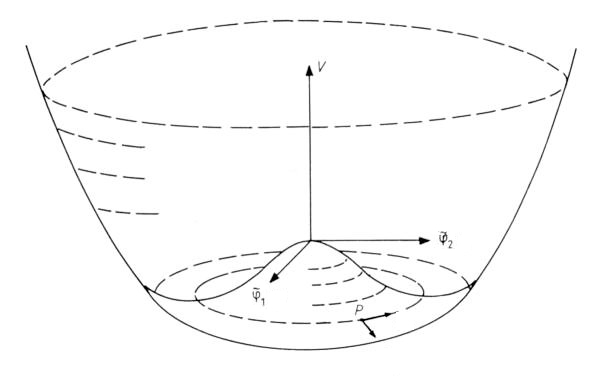
\includegraphics[width=0.5\textwidth]{images/mexicanHat.jpg}
  	\caption[Potential]
   	{$V(\phi)$ potential with $\lambda>0$ and $\mu^{2}<0$}
	\label{fig:mexicanHat}
\end{figure}

Now that we have evaluated spontaneous breaking of 
a global gauge symmetry we can extend the formalism to the local $U(1)$ gauge symmetry.
First, we make the Lagrangian (\ref{eq:LU1}) invariant under a $U(1)$ 
local gauge transformation: $\phi\rightarrow e^{i\alpha(x)}\phi$
This is done by choosing a modified derivative, $D_{\mu}$, which will
transform covariantly under phase transformations, namely, 
$D_{\mu}\rightarrow e^{i\alpha(x)}D_{\mu}\psi$. Thus $\partial_{\mu}$
is replaced by $D_{\mu} = \partial_{\mu}-ieA_{\mu}$.
The gauge invariant Lagrangian in this instance is thus,
\begin{equation}
\La=(\partial^{\mu}+ieA^{\mu})\phi*(\partial_{\mu}-ieA_{\mu})\phi - \mu^{2} \phi*\phi - \lambda(\phi*\phi)^{2}-\frac{1}{4}F_{\mu\nu}F^{\mu\nu}.
\end{equation}
To avoid off diagonal terms, instead of making the transformation (\ref{eq:VTerms})
we transform $\phi$ as,
\begin{equation}
\phi\rightarrow\sqrt{\frac{1}{2}}(\nu+h(x))e^{i\Theta(x)/\nu}
\end{equation}
and for the field $A_{\mu}$,
\begin{equation}
A_{\mu}\rightarrow A_{\mu}+\frac{1}{e\nu}\partial_{\mu}\Theta
\end{equation}
Then by translating this field to a true global minimum
and, again, considering the solution where $\mu^{2}<0$ $\lambda>0$ this Lagrangian becomes 
\begin{equation}
\La'=\frac{1}{2}(\partial_{\mu}h)^{2}-\lambda \nu^{2}h^{2}+\frac{1}{2}e^{2}\nu^{2}A_{\mu}^{2}-\lambda\nu h^{3}-
\frac{1}{4}\lambda h^{4} + \frac{1}{2}e^{2}A_{\mu}^{2}h^{2}+\nu e^{2}A_{\mu}^{2}h-\frac{1}{4}F_{\mu\nu}F^{\mu\nu}
\end{equation}
This equation describes the interaction between a vector gauge boson,
$A_{\mu}$, and a massive scalar, h. 
It is of importance to note that when examining this equation 
we see that the second term relates the mass 
of the higgs as $m_{h}=\sqrt{2\lambda v^{2}}$. 
To summarize, this example of spontaneous breaking of a $U(1)$ gauge symmetry
results in a massless Goldstone boson which has been converted to an
additional longitudinal polarization degree of freedom. This results
in a Lagrangian with a massive scalar particle, a massive field and interaction terms.
This procedure is known as the Higgs mechanism. 

Next we consider spontaneous breaking of a $SU(2)$ gauge symmetry.
We begin with (\ref{eq:LU1}) and define $\phi$ as an $SU(2)$ doublet 
of a complex scalar field, 
\begin{equation}
\phi=\left(
    \begin{array}{c}
      \phi_{\alpha} \\
      \phi_{\beta}
    \end{array}
  \right) =
  \sqrt{\frac{1}{2}} 
  \left(
    \begin{array}{c}
      \phi_{1}+i\phi_{2} \\
      \phi_{3}+i\phi_{4}
    \end{array}
  \right) .
  \label{eq:phidoublet}
\end{equation}
We must replace $\partial_{\mu}$ by the covariant derivative,
\begin{equation}
D_{\mu}=\partial_{\mu}+ig\frac{\tau_{a}}{2}W_{\mu}^{a}.
\end{equation}
The gauge invariant Lagrangian finally becomes,
\begin{equation}
\La=
\left(\partial_{\mu}\phi + ig \frac{1}{2} \tau \cdot W_{\mu}\phi  \right)^{\dagger}
\left(\partial^{\mu}\phi + ig \frac{1}{2} \tau \cdot W^{\mu}\phi  \right)
-\mu^{2}\phi^{\dagger}\phi
-\lambda (\phi^{\dagger}\phi)^{2}
-\frac{1}{4}W_{\mu\nu}W^{\mu\nu}.
\label{eq:SU2L}
\end{equation}
Here, three gauge fields $W_{\mu}^{a}$ with a = 1,2,3 are included.
The potential in this Lagrangian is $V(\phi)=\mu^{2}\phi^{\dagger}\phi+\lambda (\phi^{\dagger}\phi)^{2}$.
As before, we are interested in the global minimum of this potential
in the case where $\mu^{2}<0$ and $\lambda>0$, which is
$\phi^{\dagger}\phi=-\mu^{2}/2\lambda$, and then we expand about a point in $\phi(x)$ that is a global minimum,
\begin{equation}
\phi_{0}=\sqrt{\frac{1}{2}}
\left(
\begin{array}{c}
      0 \\
      \nu
    \end{array}
\right)
\label{eq:min}
\end{equation}
Due to gauge invariance, one can simply substitute,
\begin{equation}
\phi(x)=\sqrt{\frac{1}{2}}
\left(
\begin{array}{c}
      0 \\
      \nu+h(x)
    \end{array}
\right)
\label{eq:min}
\end{equation}
And in fact, if we substitute ($\ref{eq:min}$) into the Lagrangian (\ref{eq:SU2L}).
we find that the three bosons acquire a mass of $M=\frac{1}{2}g\nu$.

Finally, we need to formulate the Higgs mechanism in an $SU(2)\times U(1)$ 
gauge invariant Lagrangian so that the $W^{\pm}$ and $Z$ become massive. 
\begin{equation} %%link this to 14.65
\left| \left( i\partial_{\mu}+gT_{a}W_{\mu}^{1}+g'B_{\mu}\frac{Y}{2}\right)\phi \right|^{2} - \mu^{2}\left| \phi \right| ^{2}
-\lambda\left| \phi \right| ^{4}
\label{eq:L2}
\end{equation}
%%%%delete
We wish for (\ref{eq:L2}) to remain gauge invariant and 
for this Lagrangian to break the symmetries of $SU(2)$ and $U(1)_{Y}$
but leave $U(1)_{em}$, with generator $Q=T^{3}+\frac{Y}{2}$, unbroken. 
We can then make the same choice of (\ref{eq:phidoublet}) and require a vacuum 
expectation value of (\ref{eq:min}).
%then
%we choose $\phi$ such that,
%\begin{equation}
%\phi = 
%\left(
%\begin{array}{c}
%      \phi^{+} \\
%      \phi^{0}
%    \end{array}
%\right)
%\mathrm{where,}
%\begin{array}{c}
%      \phi^{+}\equiv (\phi_{1}+i\phi_{2})/\sqrt{2} \\
%      \phi^{0}\equiv (\phi_{3}+i\phi_{4})/\sqrt{2}
%    \end{array}
%\end{equation}
%%%deleted
Expanding the kinetic term of (\ref{eq:L2}) we have,
\begin{equation}
\left| \left(-g\frac{\tau}{2}\cdot W_{\mu}-i\frac{g'}{2}B_{\mu}\right)\phi\right|^{2}
\end{equation}
Then evaluating at (\ref{eq:min}),
\begin{equation}
=\frac{1}{8}\left|
\begin{pmatrix}
		gW_{\mu}^{3}+g'B_{\mu} & g(W_{\mu}^{1}-iW_{\mu}^{2})\\
		g(W_{\mu}^{1}+iW_{\mu}^{2}) & -gW_{\mu}^{3}+g'B_{\mu}
\end{pmatrix}
\begin{pmatrix}
0\\
\nu
\end{pmatrix}
\right|^{2}
\end{equation}
\begin{equation}
=
\frac{1}{8}v^{2}g^{2}\left[\left(W_{\mu}^{1} \right)^{2} \left(W_{\mu}^{2} \right)^{2} \right]
+\frac{1}{8}v^{2}(g'B_{\mu}-gW_{\mu}^{3})(g'B^{\mu}-gW^{3\mu}) 
\end{equation}
\begin{equation}
=(\frac{1}{2}v g)W_{\mu}^{+}W^{-\mu}+\frac{1}{8}(W_{\mu}^{3},B_{\mu})
\begin{pmatrix}
g^{2} & -gg'\\
-gg'  & g'^{2}
\end{pmatrix}
\begin{pmatrix}
W^{3\mu}\\
B^{\mu}
\end{pmatrix}
\label{eq:finalH}
\end{equation}
We then can obtain the masses of the vector bosons.
From the first term in in (\ref{eq:finalH}) we can then determine the 
mass of the $W$ boson, 
\begin{equation}
M_{W}=\frac{1}{2}v g.
\end{equation}
By diagonalizing the matrix on the last term of (\ref{eq:finalH}), we find that
the field associated to $Z_{\mu}$ is,
\begin{equation}
Z_{\mu}= \frac{gW_{\mu}^{3}-g'B_{\mu}}{\sqrt{g^{2}+g'^{2}}}
\end{equation}
and therefore we have,
\begin{equation}
M_{Z}=\frac{1}{2}v\sqrt{g^{2}g'^{2}}.
\end{equation}
While it is not required in the standard model that the higgs boson 
also gives mass to the fermions, it is possible and would be a nice
feature. If this were true then the coupling strength to each of the fermions
to the higgs boson would be proportional to their mass.

To generate (for example) the $\tau$ mass we construct a 
Lagrangian that is $SU(2)\times U(1)$ gauge invariant,

\begin{equation}
\La = -G_{\tau}\left[
      (\bar{\nu_{\tau}},\bar{\tau})_{L}
	\left( \begin{array}{c}
      \phi^{+} \\
      \phi^{-}
      \end{array}\right)\tau_{R} 
    +
      \bar{\tau}_{R}(\phi^{-},\bar{\phi^{0}})
	\left( \begin{array}{c}
      \nu_{e} \\
      e
      \end{array}\right)_{L}
    \right]
\end{equation}
Substituting in
\begin{equation}
\phi=\sqrt{\frac{1}{2}}
\left( \begin{array}{c}
      0 \\
      \nu + h(x)
      \end{array}\right)
\end{equation}
This leads to,
\begin{equation}
\La = -\frac{G_{\tau}}{\sqrt{2}}\nu(\bar{\tau}_{L}\tau_{R}+\bar{\tau}_{R}\tau_{L})
-\frac{G_{\tau}}{\sqrt{2}}(\bar{\tau}_{L}\tau_{R}+\bar{\tau}_{R}\tau_{L})h.
\end{equation}
Then the masses of the fermions can be obtained by choosing $G_{e}$ such that,
\begin{equation}
m_{e}=\frac{G_{e}\nu}{\sqrt{2}}
\end{equation}
The recent evidence of $h$ coupling to $\tau\tau$ (REFERENCE PAPER) suggests
that the higgs mechanism could be used to give mass to the fermions, however,
it is not required and more measurements will need to be performed.

%%%%%subsection
\subsection{W Boson Production}
\begin{figure}[t]
\centering
  \begin{subfigure}[b]{.35\textwidth}
	\marginbox{-10mm 0pt 10mm 0pt}{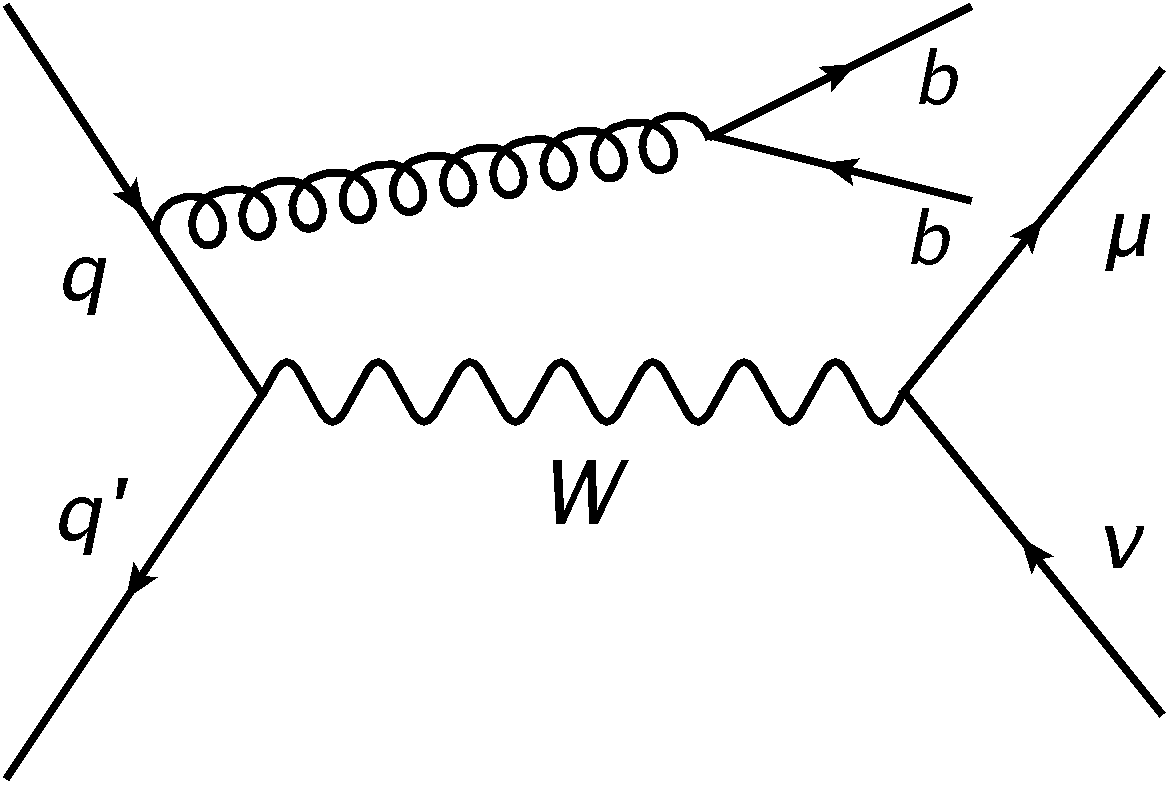
\includegraphics[width=\textwidth]{images/Wbb1.png} }
	\end{subfigure}	
   \begin{subfigure}[b]{.35\textwidth}
	\marginbox{10mm 0pt -10mm 0pt}{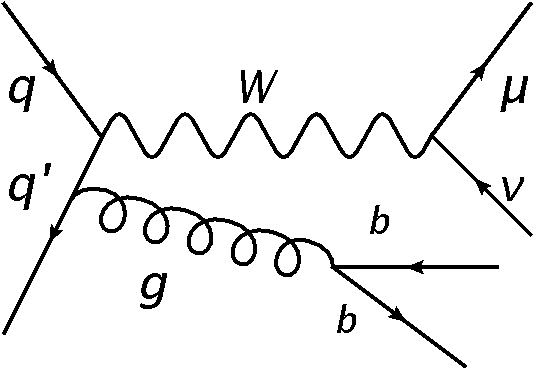
\includegraphics[width=\textwidth]{images/Wbb2.png}}
    \end{subfigure}	
  	\caption[Leading Order $\Wbb$ diagrams]
   	{Leading Order $\Wbb$ diagrams}

	\label{fig:WbbLO}
\end{figure}

In a hadron collider, such as the LHC, W bosons are primarily produced
through the annihilation of a quark (Q=$\pm\frac{2}{3}$) and an anti-quark (Q=$\pm\frac{1}{3}$). 
%The coupling of quarks and leptons to $W^{\pm}$ has a pure V-A form.
Experimentally it has been determined that W coupling is favored within quark generations,
$u\bar{d}\rightarrow W^{+}$,
and suppressed, although not 0, across generations, $s\bar{u}\rightarrow W^{-}$.
This has been paramaterized by introducing 'Cabibbo-rotated' states, 
\begin{equation}
\left(
    \begin{array}{c}
      u \\
      d' 
    \end{array}
  \right),
  \left(
    \begin{array}{c}
      c \\
      s' 
    \end{array}
  \right),
\left(
    \begin{array}{c}
      t \\
      b' 
    \end{array}
  \right)  
\end{equation}
where there is no mixing across states and ($d',s',b'$) are composites
of ($d,s,b$). Namely,
\begin{equation}
\left(
    \begin{array}{c}
      d' \\
      s'  \\
      b'
    \end{array}
  \right)
  =
  \begin{pmatrix}
  V_{ud} & V_{us} & V_{ub}\\
  V_{cd} & V_{cs} & V_{cb}\\
  V_{td} & V_{ts} & V_{tb}
  \end{pmatrix}
  =
  \left(
    \begin{array}{c}
      d \\
      s  \\
      b
    \end{array}
  \right)
\end{equation}
%\begin{equation}
%J^{\mu}=(\bar{u},\bar{c},\bar{t})\frac{\gamma_}{}
%\end{equation}
%This has been neatly summarized into a $3\times3$ matrix, 
%the Cabbibo-Kobayashi-Maskawa matrix which relates
%the coupling strength of the quarks via the charged current.
%The Cabibbo Kobayashi Maskawa (CKM) matrix tells us that%%More on CKM matrix
The matrix {\bf V} is written in terms of three generalized Cabbibo angles.
The standard model provides no way to calculate the weak mixing angles, instead they
are taken from data.
%This effect is extremely important
%when considering W production at hadron colliders and in b quark physics. 
With this effect in mind we can write the matrix element for W production through quark fusion.
Neglecting the mass of the quarks, spins and the W polarization, the matrix element is,
\begin{equation}
\sum|M|^{2}=|V_{qq'}|^{2}\frac{8G_{F}}{\sqrt{2}}M_{W}^{4}
\end{equation}
The above equation is summed over all quarks, $qq'$. The cross section for W production is,
\begin{equation}
\sigma=2\times2\pi\frac{G_{F}}{\sqrt{2}}M_{W}^{2}|V_{qq'}|^{2}\delta(s-M_{W}^{2})
\end{equation}
Where s is the center of mass energy squared of the two partons, $s=(p_{1}+p_{2})^{2}$.
Importantly, the term $\delta(s-M_{W}^{2})$ leads us to the 
conclusion that incoming quarks are required to have a center of mass energy
equal to the mass of the W. 
In 2011 at the LHC protons were collided with an energy of $\sqrt{S}=7$ TeV, and 8 TeV in 2012.
For a W boson to be created two interacting partons must have suitable
momentum fractions $x, y$ such that $(x+y)S=s$.
In lepton-positron colliders, $W$ bosons are produced in pairs when 
the center of mass energy reaches a threshold of 161 $GeV$. 
\begin{equation}
\sigma=2\times\frac{2\pi G_{F}}{3\sqrt{2}}\int{dxdy \sum{V_{q,\bar{q}'}}xyS f_{q}(x)f_{\bar{q}'}(y)}
\end{equation}
The branching ratio of the $W$ to $\mu$ $\nu$, as predicted by theory, is approximately 0.11. 

As shown in Figure \ref{fig:WbbLO}, the $\Wbb$ process at leading order requires that one of the initial partons
radiates a gluon and the gluon then splits into a $\bbbar$ pair. Each additional
vertex involving the gluon adds a factor of order $\alpha_{s}$. A full
calculation of the theoretical $\Wbb$ cross section at NLO can be found here \cite{Campbell:2010ff, Badger:2010mg}.
$\Wbb$ is an irreducible background to many searches including:
$hW$ where a W is produced and a higgs boson is radiated from the W
and then decays to a b quark pair, minimally supersymmetric $H,h,A\rightarrow \tau\tau$
where production is enhanced in association with b-quarks and many other beyond the standard
model searches where the final state includes a single lepton and b quarks. 
A measurement of $\Wbb$ via the $W$ decay to $\mu$ + $\nu$ is presented as a 
central focus of this thesis.

\subsection{Jet Hadronization and b-quarks}
During a high energy interaction involving quarks in the final state (for instance $g\rightarrow q\bar{q}$)
the final state quarks fly off as individual particles for a very brief moment. After they reach
a distance of ~$10^{-15}m$ the strong interaction is so great that new quarks and anti-quarks
are produced. These new quarks and anti-quarks then combine in many different combinations
to form baryons and mesons. This process is known as hadronization. Although many QCD
next to leading order calculations have been performed, hadronization can not yet be directly calculated.
Instead monte carlo event generators simulate this hadronic production using parton 
showering with various fragmentation models.%%%P170 QCD and collider physics book Parton showering produces partons of successively lower energy

If we consider a high energy parton, b, with with energy $E_{b}$ which produces a hadron, B, with energy $E_{B}$
then the hadron's energy fraction is $z=E_{B}/E_{b}$. The probability of finding B in the range
$z$ to $dz$ for a heavy b quark is,
\begin{equation}
\int{D_{b}^{B}(z)dz}=\int{\frac{Constant}{z(1-\frac{1}{z}-\frac{\epsilon_{b}}{1-z})}dz}
\end{equation}
Here $\epsilon_{b}=\langle m_{b}^{2}+ p_{T,b}^{2} \rangle/\langle m_{B}^{2}+ p_{T,B}^{2} \rangle$, and is expected to be proportional to $m_{b}^{-2}$.
In the case where the fragmenting parton is a b quark, it loses only a very small amount
of its energy to materialize a number of light quark pairs and a majority of the energy is
carried off by the B hadron.  
For comparison, the average b-meson lifetime is $1.55\pm 0.06 ps$, this corresponds to a proper lifetime of
$c\tau=463\mu m$. For a b-meson with 20$GeV$ momentum this would correspond to
1.9 $mm$ in the lab frame. Therefore a small $V_{cb}$ allows for detection of a separated vertex. 
This long lifetime is extremely helpful in distinguishing jets which
originate from b quarks from jets that originate from lighter quarks or gluons that do not produce heavy quarks. 

%\subsection{Wbb Diagrams}